\begin{figure}[H]
\centering



\tikzset{every picture/.style={line width=0.75pt}} %set default line width to 0.75pt        

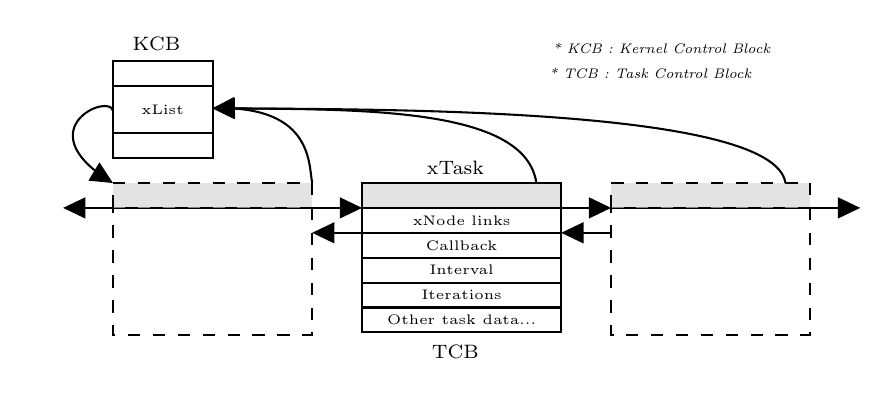
\begin{tikzpicture}[x=0.75pt,y=0.75pt,yscale=-1,xscale=1,scale=1.2]
%uncomment if require: \path (0,300); %set diagram left start at 0, and has height of 300

%Shape: Rectangle [id:dp7393772911700529] 
\draw   (220,99) -- (300,99) -- (300,109) -- (220,109) -- cycle ;
%Shape: Rectangle [id:dp3269756667152006] 
\draw  [fill={rgb, 255:red, 210; green, 210; blue, 210 }  ,fill opacity=0.62 ] (220,79) -- (300,79) -- (300,89) -- (220,89) -- cycle ;
%Straight Lines [id:da8437617817918501] 
\draw    (220,99) -- (203,99) ;
\draw [shift={(200,99)}, rotate = 360] [fill={rgb, 255:red, 0; green, 0; blue, 0 }  ][line width=0.08]  [draw opacity=0] (8.93,-4.29) -- (0,0) -- (8.93,4.29) -- cycle    ;

%Shape: Rectangle [id:dp6797270650972396] 
\draw   (220,109) -- (300,109) -- (300,119) -- (220,119) -- cycle ;
%Shape: Rectangle [id:dp7082925742154869] 
\draw   (220,119) -- (300,119) -- (300,129) -- (220,129) -- cycle ;
%Shape: Rectangle [id:dp07500883444191397] 
\draw  [dash pattern={on 4.5pt off 4.5pt}] (320,89) -- (400,89) -- (400,140) -- (320,140) -- cycle ;
%Shape: Rectangle [id:dp1655091650065761] 
\draw  [fill={rgb, 255:red, 210; green, 210; blue, 210 }  ,fill opacity=0.62 ][dash pattern={on 4.5pt off 4.5pt}] (320,79) -- (400,79) -- (400,89) -- (320,89) -- cycle ;
%Shape: Rectangle [id:dp41731190816610786] 
\draw   (220,129) -- (300,129) -- (300,139) -- (220,139) -- cycle ;
%Shape: Rectangle [id:dp7128391239392147] 
\draw  [dash pattern={on 4.5pt off 4.5pt}] (120,89) -- (200,89) -- (200,140) -- (120,140) -- cycle ;
%Shape: Rectangle [id:dp6294241444639113] 
\draw  [fill={rgb, 255:red, 210; green, 210; blue, 210 }  ,fill opacity=0.62 ][dash pattern={on 4.5pt off 4.5pt}] (120,79) -- (200,79) -- (200,89) -- (120,89) -- cycle ;
%Straight Lines [id:da7035500548577738] 
\draw    (200,89) -- (217,89) ;
\draw [shift={(220,89)}, rotate = 180] [fill={rgb, 255:red, 0; green, 0; blue, 0 }  ][line width=0.08]  [draw opacity=0] (8.93,-4.29) -- (0,0) -- (8.93,4.29) -- cycle    ;

%Shape: Rectangle [id:dp6948885007559562] 
\draw   (220,89) -- (300,89) -- (300,99) -- (220,99) -- cycle ;
%Straight Lines [id:da15424177619276613] 
\draw    (320,99) -- (303,99) ;
\draw [shift={(300,99)}, rotate = 360] [fill={rgb, 255:red, 0; green, 0; blue, 0 }  ][line width=0.08]  [draw opacity=0] (8.93,-4.29) -- (0,0) -- (8.93,4.29) -- cycle    ;

%Straight Lines [id:da2528678866806362] 
\draw    (300,89) -- (317,89) ;
\draw [shift={(320,89)}, rotate = 180] [fill={rgb, 255:red, 0; green, 0; blue, 0 }  ][line width=0.08]  [draw opacity=0] (8.93,-4.29) -- (0,0) -- (8.93,4.29) -- cycle    ;

%Straight Lines [id:da6291496971915145] 
\draw    (120,89) -- (103,89) ;
\draw [shift={(100,89)}, rotate = 360] [fill={rgb, 255:red, 0; green, 0; blue, 0 }  ][line width=0.08]  [draw opacity=0] (8.93,-4.29) -- (0,0) -- (8.93,4.29) -- cycle    ;

%Straight Lines [id:da0516312905093983] 
\draw    (400,89) -- (417,89) ;
\draw [shift={(420,89)}, rotate = 180] [fill={rgb, 255:red, 0; green, 0; blue, 0 }  ][line width=0.08]  [draw opacity=0] (8.93,-4.29) -- (0,0) -- (8.93,4.29) -- cycle    ;

%Shape: Rectangle [id:dp12186802276532593] 
\draw   (120,30) -- (160,30) -- (160,40) -- (120,40) -- cycle ;
%Shape: Rectangle [id:dp8210016213305442] 
\draw   (120,40) -- (160,40) -- (160,59) -- (120,59) -- cycle ;
%Shape: Rectangle [id:dp20074469318358568] 
\draw   (120,59) -- (160,59) -- (160,69) -- (120,69) -- cycle ;
%Curve Lines [id:da9811819988198454] 
\draw    (290,79) .. controls (285.57,48.04) and (217.59,49.52) .. (162.51,49.02) ;
\draw [shift={(160,49)}, rotate = 360.59000000000003] [fill={rgb, 255:red, 0; green, 0; blue, 0 }  ][line width=0.08]  [draw opacity=0] (8.93,-4.29) -- (0,0) -- (8.93,4.29) -- cycle    ;

%Curve Lines [id:da5106049490604561] 
\draw    (200,79) .. controls (198.54,71.76) and (200.4,48.76) .. (162.96,48.94) ;
\draw [shift={(160,49)}, rotate = 357.98] [fill={rgb, 255:red, 0; green, 0; blue, 0 }  ][line width=0.08]  [draw opacity=0] (8.93,-4.29) -- (0,0) -- (8.93,4.29) -- cycle    ;

%Curve Lines [id:da11501986334214753] 
\draw    (390,79) .. controls (385.57,48.04) and (220.56,49.52) .. (162.57,49.02) ;
\draw [shift={(160,49)}, rotate = 360.59000000000003] [fill={rgb, 255:red, 0; green, 0; blue, 0 }  ][line width=0.08]  [draw opacity=0] (8.93,-4.29) -- (0,0) -- (8.93,4.29) -- cycle    ;

%Curve Lines [id:da3794145473394166] 
\draw    (120,50) .. controls (118.54,42.76) and (86.18,56.84) .. (117.47,77.41) ;
\draw [shift={(120,79)}, rotate = 211.12] [fill={rgb, 255:red, 0; green, 0; blue, 0 }  ][line width=0.08]  [draw opacity=0] (8.93,-4.29) -- (0,0) -- (8.93,4.29) -- cycle    ;


% Text Node
\draw (260,104) node  [font=\tiny] [align=left] {Callback};
% Text Node
\draw (260,114) node  [font=\tiny] [align=left] {Interval};
% Text Node
\draw (260,124) node  [font=\tiny] [align=left] {Iterations};
% Text Node
\draw (260,134) node  [font=\tiny] [align=left] {Other task data...};
% Text Node
\draw (257.5,147) node  [font=\scriptsize] [align=left] {TCB};
% Text Node
\draw (260,94) node  [font=\tiny] [align=left] {xNode links};
% Text Node
\draw (137.5,23) node  [font=\scriptsize] [align=left] {KCB};
% Text Node
\draw (140,49.5) node  [font=\tiny] [align=left] {xList};
% Text Node
\draw (257.5,73) node  [font=\scriptsize] [align=left] {xTask};
% Text Node
\draw (340.5,25) node  [font=\tiny] [align=left] {\textit{* KCB : Kernel Control Block}};
% Text Node
\draw (336,35) node  [font=\tiny] [align=left] {\textit{* TCB : Task Control Block}};


\end{tikzpicture}

\caption{Task node illustration}
\label{fig:tasklist}
\end{figure}
